\section{Introduction}
\label{sec:intro}

\begin{figure}[t]
\centering
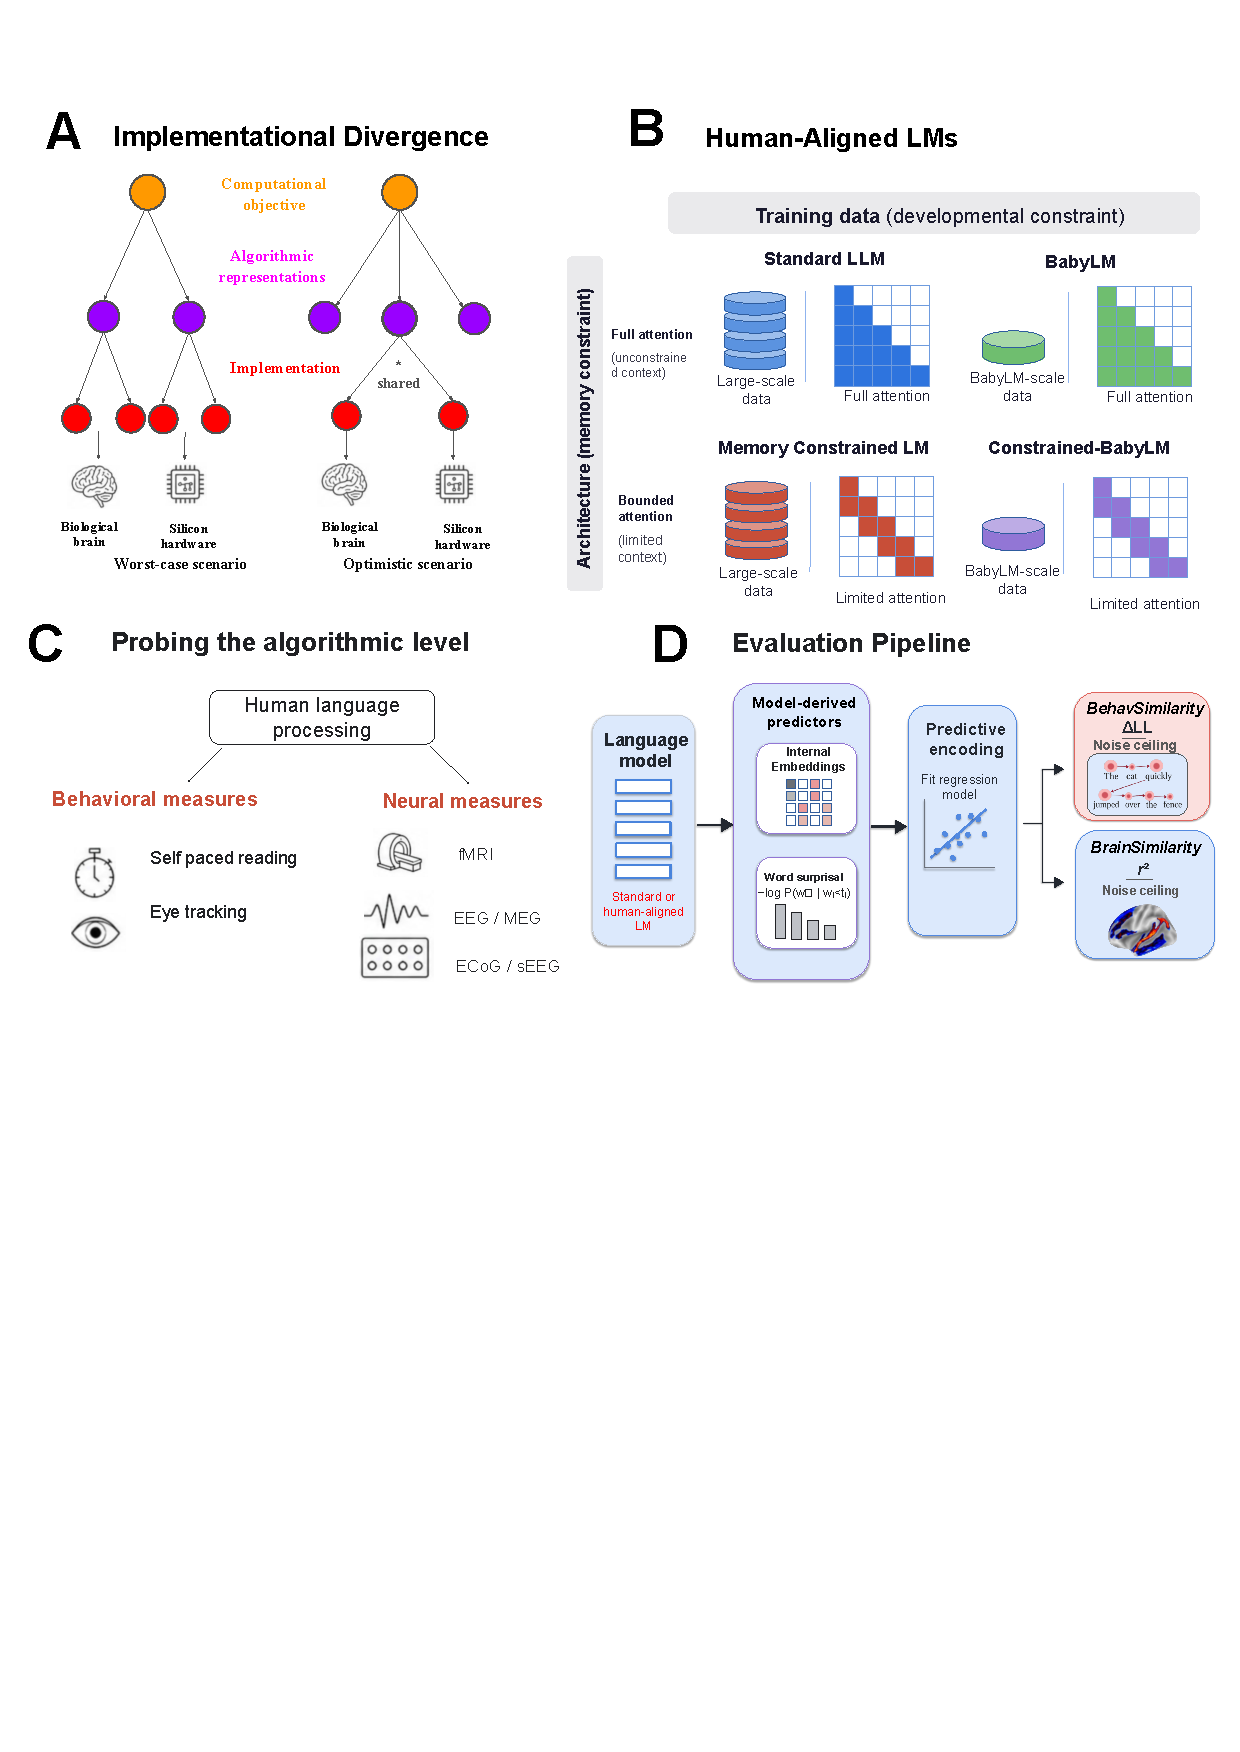
\includegraphics[page=1,trim=4 365 4 37,clip,width=\textwidth]{figures/humanscore_figures.pdf}
\caption{Overview. (A) In Marr's framework, humans and LLMs may share algorithmic-level representations even though they differ at the computational and implementational levels. (B) Human-aligned models add a memory constraint (bounded attention), a developmental data constraint (BabyLM-scale training), or both, to the standard LLM recipe; crossing the two gives four model groups. (C) Human processing is probed with behavioral (self-paced reading, eye-tracking) and neural (fMRI, EEG/MEG, ECoG) measures. (D) Each model is scored against each human dataset; scores are normalized by the reliability of the human data and summarized as brain similarity and behavioral similarity.}
\label{fig:overview}
\end{figure}

Large language models (LLMs) predict human brain responses to language \citep{schrimpf2021neural,caucheteux2022brains} and word-by-word reading times \citep{goodkind2018predictive,wilcox2020predictive} surprisingly well. They do so, however, with a computational recipe that is far from human (Figure~\ref{fig:overview}A; \citealp{marr1982vision}): global attention over thousands of tokens and training on trillions of words, several orders of magnitude more than a child hears \citep{gilkerson2017mapping,warstadt2023cfp}. Two lines of work have tried to close this gap. Psycholinguists build memory limits into the architecture, motivated by capacity-limited accounts of sentence processing \citep{lewisvasishth2005activation,futrell2020lossy}: attention biased toward recent words \citep{press2021train,devarda2024locally,clark2025linear}, forget gates \citep{lin2025forgetting}, bounded recurrent states \citep{timkey2023limited} or hard context windows \citep{bu2026staticlinearattentionconstraints}. The BabyLM Challenge restricts training to 10--100 million words, a developmentally plausible budget \citep{warstadt2023findings,hu2024secondbabylm}. Both share an assumption: a model that works under human constraints should process language more like humans.

This assumption is rarely tested against both kinds of human data at once, and the two need not agree. Reading times index the moment-to-moment difficulty of a word, which surprisal predicts \citep{hale2001probabilistic,levy2008expectation}, and smaller or less accurate models often predict it better \citep{ohschuler2023why,kuribayashi2021lower}. Brain responses reflect rich contextual representations, which larger models tend to match better \citep{schrimpf2021neural,caucheteux2022brains}. A constraint could therefore help on one side and not on the other. Testing this also requires separating the constraint from scale: constrained models are small and have high perplexity, both of which change alignment on their own.

We build a benchmark that places 118 models in a $2\times2$ design (Figure~\ref{fig:overview}B): memory-constrained or standard architectures, trained on web-scale or BabyLM-scale data. Each model is compared with 16 reading-time measures from self-paced reading and eye-tracking and with eight neural datasets spanning fMRI, EEG, MEG and intracranial recordings (Figure~\ref{fig:overview}C). We score models by representational similarity \citep{kriegeskorte2008rsa}: how much a model's dissimilarity matrix over words improves the held-out prediction of the human one beyond word length and frequency (Figure~\ref{fig:method}A). The model enters through a single coefficient, so the score cannot grow with the width of a learned mapping, unlike encoding scores \citep{alkhamissi-etal-2025-language}. A mixed-effects regression across models then estimates each constraint's association with similarity at matched size and perplexity, with model families as a source of dependence, and its estimates are checked by adding 119 intermediate training checkpoints of Pythia and of a BabyLM GPT-2 baseline that fill the perplexity range in which constrained and standard models do not overlap.

Our findings are:
\begin{itemize}
    \item \textbf{Constraints go with behavioral, not brain, similarity.} At matched size and perplexity, both the memory and the data constraint are associated with higher similarity to reading behavior. Neither is associated with higher brain similarity, where large standard LLMs lead (Section~\ref{sec:results-main}).
    \item \textbf{Syntactic memory load gives only a weak test of the memory constraint.} On words that close long dependencies \citep{gibson2000dlt}, both constraints are associated with higher behavioral similarity, but not reliably more than on easy words. Once length and frequency are controlled, these words slow readers in only one corpus, Natural Stories, and by a third of the cost of a rare word, so these corpora give too little DLT-related cost for a strong test (Section~\ref{sec:results-dlt}).
    \item \textbf{It is about rare words.} In units of the human reliability, the advantage of both constraints is concentrated on word pairs containing a rare word, where reading times are most informative, in the measures where rare words separate models most (Section~\ref{sec:results-freq}).
    \item \textbf{No advantage on the multiple-demand network.} The domain-general network that supports working memory \citep{duncan2010multiple} is predicted poorly by every model, and constrained models do not match it better than standard LLMs (Section~\ref{sec:results-md}).
\end{itemize}
